%%%%%%%%%%%%%%%%%%%%%%%%%%%%%%%%%%%%%%%%%%%%%%%%%%%%%%%%%%%%%%%%%%%%%%%

\chapter{Experiment 3: Signal Generation and Digital-to-Analogue Conversion}

This chapter presents the implementation of an 8-bit Arduino Function Generator using an R-2R DAC, operational amplifier, and RC filter. The experiment demonstrates the generation of sine, square, and triangle waveforms using Direct Digital Synthesis (DDS), along with frequency and amplitude control through potentiometers.

%%%%%%%%%%%%%%%%%%%%%%%%%%%%%%%%%%%%%%%%%%%%%%%%%%%%%%%%%%%%%%%%%%%%%%%

\section{8-Bit Arduino Function Generator using DAC and Op-Amp}

%%%%%%%%%%%%%%%%%%%%%%%%%%%%%%%%%%%%%%%%%%%%%%%%%%%%%%%%%%%%%%%%%%%%%%%

\subsection{Project Name}

8-Bit Arduino Function Generator using DAC and Op-Amp

%%%%%%%%%%%%%%%%%%%%%%%%%%%%%%%%%%%%%%%%%%%%%%%%%%%%%%%%%%%%%%%%%%%%%%%

\subsection{Problem Statement}

This experiment demonstrates waveform generation using Arduino UNO, an 8-bit R-2R DAC, operational amplifier, and RC filter.

The system generates sine, square, and triangle waveforms using the Direct Digital Synthesis (DDS) technique. Frequency and amplitude of the generated signals can be adjusted using potentiometers, while an SSD1306 OLED display provides real-time information about the selected waveform and control parameters.

%%%%%%%%%%%%%%%%%%%%%%%%%%%%%%%%%%%%%%%%%%%%%%%%%%%%%%%%%%%%%%%%%%%%%%%

\subsection{Components Used \& Pin Connections}

\begin{table}[H]
\centering

\begin{minipage}[t]{0.48\textwidth}
\centering
\caption{Function Generator Components}
\label{tab:function_components}

\begin{tabular}{|p{4cm}|c|}
\hline
\textbf{Component} & \textbf{Quantity} \\
\hline
Arduino UNO & 1 \\
8-Bit R-2R DAC & 1 \\
SSD1306 OLED Display & 1 \\
Operational Amplifier & 1 \\
10k Potentiometer & 2 \\
Push Switch & 4 \\
Resistors & Multiple \\
Capacitor & 1 \\
Oscilloscope & 1 \\
\hline
\end{tabular}

\end{minipage}
\hfill
\begin{minipage}[t]{0.47\textwidth}
\centering
\caption{Control Connections}
\label{tab:function_control}

\begin{tabular}{|l|c|}
\hline
\textbf{Device} & \textbf{Arduino Pin} \\
\hline
Power Switch & D8 \\
Sine Wave Switch & D9 \\
Square Wave Switch & D10 \\
Triangle Wave Switch & D11 \\
Frequency Potentiometer & A0 \\
Amplitude Potentiometer & A1 \\
OLED SDA & A4 \\
OLED SCL & A5 \\
\hline
\end{tabular}

\end{minipage}

\end{table}

%%%%%%%%%%%%%%%%%%%%%%%%%%%%%%%%%%%%%%%%%%%%%%%%%%%%%%%%%%%%%%%%%%%%%%%

\subsection{DAC Connections}

\begin{table}[H]
\centering
\caption{8-Bit DAC Connections}
\label{tab:dac_connections}

\begin{tabular}{|c|c|}
\hline
\textbf{DAC Pin} & \textbf{Arduino Pin} \\
\hline
D0 & D0 \\
D1 & D1 \\
D2 & D2 \\
D3 & D3 \\
D4 & D4 \\
D5 & D5 \\
D6 & D6 \\
D7 & D7 \\
\hline
\end{tabular}

\end{table}

%%%%%%%%%%%%%%%%%%%%%%%%%%%%%%%%%%%%%%%%%%%%%%%%%%%%%%%%%%%%%%%%%%%%%%%

\subsection{Software Used}

\begin{itemize}
    \item Arduino IDE
    \item SimulIDE
\end{itemize}

%%%%%%%%%%%%%%%%%%%%%%%%%%%%%%%%%%%%%%%%%%%%%%%%%%%%%%%%%%%%%%%%%%%%%%%

\subsection{Circuit Diagram}

\begin{figure}[H]
\centering

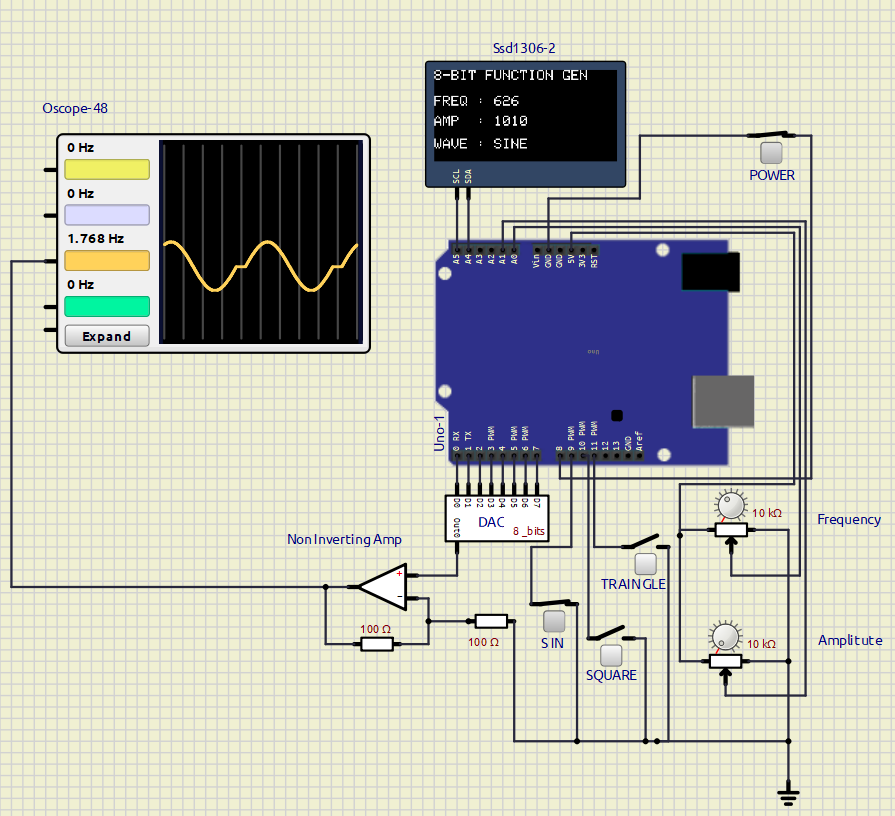
\includegraphics[width=0.65\textwidth]{Exp-3/signal_gen/sin_wave.png}

\caption{8-Bit Arduino Function Generator Circuit Diagram}
\label{fig:function_generator}

\end{figure}

%%%%%%%%%%%%%%%%%%%%%%%%%%%%%%%%%%%%%%%%%%%%%%%%%%%%%%%%%%%%%%%%%%%%%%%

\subsection{Source Code}

The complete Arduino source code for this experiment is available in the project repository.

\href{https://github.com/YOUR_USERNAME/YOUR_REPOSITORY/blob/main/Exp-3/function_generator/function_generator.ino}
{\textbf{Click here to view the Arduino Source Code}}

%%%%%%%%%%%%%%%%%%%%%%%%%%%%%%%%%%%%%%%%%%%%%%%%%%%%%%%%%%%%%%%%%%%%%%%
%%%%%%%%%%%%%%%%%%%%%%%%%%%%%%%%%%%%%%%%%%%%%%%%%%%%%%%%%%%%%%%%%%%%%%%

\subsection{Working Principle}

\begin{enumerate}

\item Arduino UNO continuously reads the frequency and amplitude values from two potentiometers.

\item The user selects the desired waveform (Sine, Square, or Triangle) using dedicated push switches.

\item A 256-sample sine lookup table is stored in memory for efficient sine wave generation using the Direct Digital Synthesis (DDS) technique.

\item Arduino outputs 8-bit digital data through PORTD (D0--D7).

\item The R-2R DAC converts the digital values into corresponding analog voltage levels.

\item The operational amplifier buffers the DAC output and improves signal stability.

\item An RC low-pass filter smooths the staircase DAC output to produce a cleaner analog waveform.

\item The generated waveform is observed on an oscilloscope, while the OLED display continuously shows the selected waveform, frequency, and amplitude values.

\end{enumerate}

%%%%%%%%%%%%%%%%%%%%%%%%%%%%%%%%%%%%%%%%%%%%%%%%%%%%%%%%%%%%%%%%%%%%%%%

\subsection{Output}

\begin{figure}[H]
\centering

\begin{minipage}{0.31\textwidth}
\centering
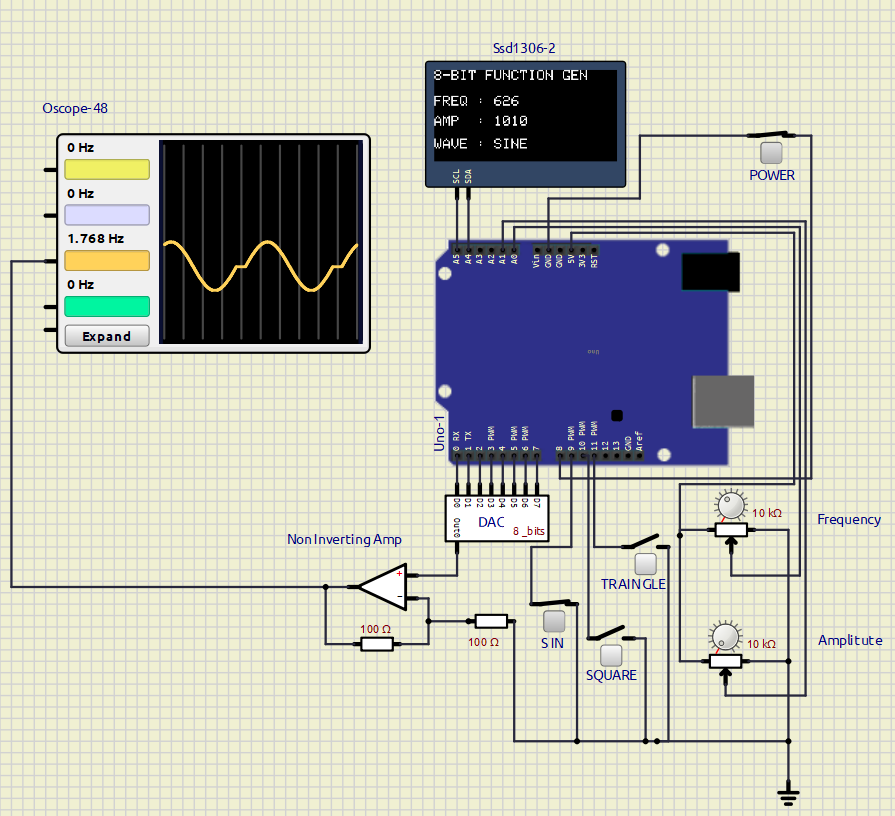
\includegraphics[width=\linewidth]{Exp-3/signal_gen/sin_wave.png}
\\
\small (a) Sine Wave
\end{minipage}
\hfill
\begin{minipage}{0.31\textwidth}
\centering
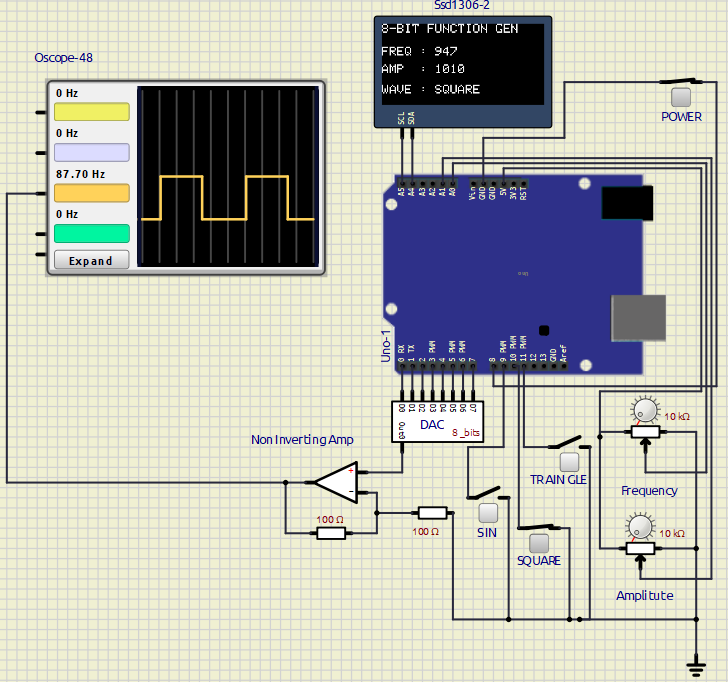
\includegraphics[width=\linewidth]{Exp-3/signal_gen/square.png}
\\
\small (b) Square Wave
\end{minipage}
\hfill
\begin{minipage}{0.31\textwidth}
\centering
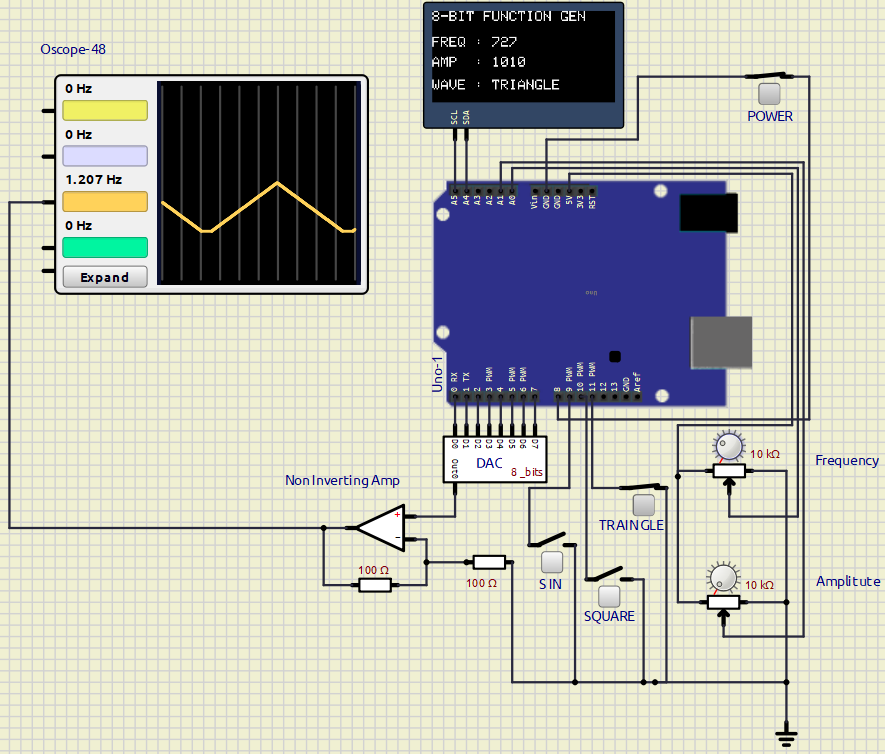
\includegraphics[width=\linewidth]{Exp-3/signal_gen/Traingle_wave.png}
\\
\small (c) Triangle Wave
\end{minipage}

\caption{Generated Waveforms of the 8-Bit Arduino Function Generator}
\label{fig:function_output}

\end{figure}

%%%%%%%%%%%%%%%%%%%%%%%%%%%%%%%%%%%%%%%%%%%%%%%%%%%%%%%%%%%%%%%%%%%%%%%

\subsection{Learning Outcomes}

\begin{itemize}

\item Understanding of Digital-to-Analog Conversion (DAC)

\item Direct Digital Synthesis (DDS) waveform generation

\item High-speed digital output using PORTD

\item Frequency control using timing delay

\item Waveform generation using lookup tables

\item OLED interfacing with Arduino

\item Signal conditioning using operational amplifiers and RC filters

\end{itemize}

%%%%%%%%%%%%%%%%%%%%%%%%%%%%%%%%%%%%%%%%%%%%%%%%%%%%%%%%%%%%%%%%%%%%%%%

\subsection{Conclusion}

The 8-Bit Arduino Function Generator using an R-2R DAC, operational amplifier, and RC filter was successfully designed and simulated using Arduino UNO.

The system generated sine, square, and triangle waveforms using the Direct Digital Synthesis (DDS) technique. Adjustable frequency and amplitude controls, together with OLED-based status monitoring, provided a practical understanding of waveform generation, DAC operation, signal conditioning, and embedded system programming.

%%%%%%%%%%%%%%%%%%%%%%%%%%%%%%%%%%%%%%%%%%%%%%%%%%%%%%%%%%%%%%%%%%%%%%%

\subsection{References}

\begin{enumerate}

\item Arduino Official Website

\url{https://www.arduino.cc/}

\item SSD1306 OLED Documentation

\url{https://github.com/adafruit/Adafruit_SSD1306}

\item Adafruit GFX Library

\url{https://github.com/adafruit/Adafruit-GFX-Library}

\item SimulIDE Official Website

\url{https://simulide.com/}

\item Arduino Simple Waveform Generator Tutorial

\url{https://docs.arduino.cc/tutorials/due/simple-waveform-generator/}

\end{enumerate}

%%%%%%%%%%%%%%%%%%%%%%%%%%%%%%%%%%%%%%%%%%%%%%%%%%%%%%%%%%%%%%%%%%%%%%%

\clearpage

%%%%%%%%%%%%%%%%%%%%%%%%%%%%%%%%%%%%%%%%%%%%%%%%%%%%%%%%%%%%%%%%%%%%%%%

\clearpage
Experiment 3 (Go Further 2):
\section{Arduino UNO-Based Lissajous Pattern Generator}

%%%%%%%%%%%%%%%%%%%%%%%%%%%%%%%%%%%%%%%%%%%%%%%%%%%%%%%%%%%%%%%%%%%%%%%

\subsection{Problem Statement}

This experiment demonstrates the generation and visualisation of Lissajous patterns using two sinusoidal signals and an SSD1306 OLED display.

The project helps in understanding frequency ratios, phase difference, analogue signal sampling, coordinate mapping, and graphical visualisation using Arduino UNO.

Different geometric patterns are generated when two sine waves having different frequencies and phase shifts are simultaneously applied to the X-axis and Y-axis of the display system.

%%%%%%%%%%%%%%%%%%%%%%%%%%%%%%%%%%%%%%%%%%%%%%%%%%%%%%%%%%%%%%%%%%%%%%%

\subsection{Components Used \& Pin Connections}

\begin{table}[H]
\centering

\begin{minipage}[t]{0.48\textwidth}
\centering
\caption{Lissajous Pattern Generator Components}
\label{tab:lissajous_components}

\begin{tabular}{|p{4cm}|c|}
\hline
\textbf{Component} & \textbf{Quantity} \\
\hline
Arduino UNO & 1 \\
SSD1306 OLED Display & 1 \\
Sine Wave Generator & 2 \\
Connecting Wires & Multiple \\
Oscilloscope (Optional) & 1 \\
\hline
\end{tabular}

\end{minipage}
\hfill
\begin{minipage}[t]{0.47\textwidth}
\centering
\caption{Signal Connections}
\label{tab:lissajous_connections}

\begin{tabular}{|l|c|}
\hline
\textbf{Device} & \textbf{Arduino Pin} \\
\hline
X Signal Input & A0 \\
Y Signal Input & A1 \\
OLED SDA & A4 \\
OLED SCL & A5 \\
\hline
\end{tabular}

\end{minipage}

\end{table}

%%%%%%%%%%%%%%%%%%%%%%%%%%%%%%%%%%%%%%%%%%%%%%%%%%%%%%%%%%%%%%%%%%%%%%%

\subsection{Software Used}

\begin{itemize}
    \item Arduino IDE
    \item SimulIDE
\end{itemize}

%%%%%%%%%%%%%%%%%%%%%%%%%%%%%%%%%%%%%%%%%%%%%%%%%%%%%%%%%%%%%%%%%%%%%%%

\subsection{Circuit Diagram}

\begin{figure}[H]
\centering

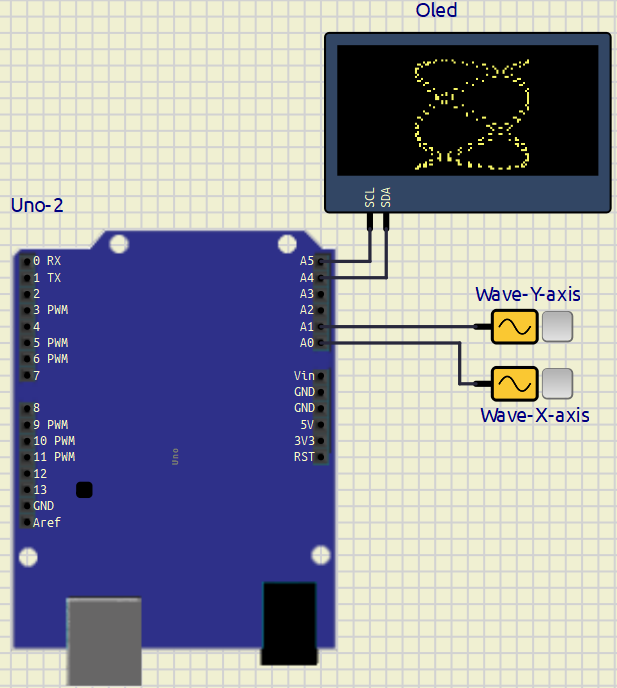
\includegraphics[width=0.60\textwidth]{Exp-3/Lissajous_pattern/circuit.png}

\caption{Arduino UNO-Based Lissajous Pattern Generator Circuit Diagram}
\label{fig:lissajous_circuit}

\end{figure}

%%%%%%%%%%%%%%%%%%%%%%%%%%%%%%%%%%%%%%%%%%%%%%%%%%%%%%%%%%%%%%%%%%%%%%%

\subsection{Source Code}

The complete Arduino source code for this experiment is available in the project repository.

\href{https://github.com/YOUR_USERNAME/YOUR_REPOSITORY/blob/main/Exp-3/Lissajous_Pattern_Generator/Lissajous_Pattern_Generator.ino}
{\textbf{Click here to view the Arduino Source Code}}

%%%%%%%%%%%%%%%%%%%%%%%%%%%%%%%%%%%%%%%%%%%%%%%%%%%%%%%%%%%%%%%%%%%%%%%
%%%%%%%%%%%%%%%%%%%%%%%%%%%%%%%%%%%%%%%%%%%%%%%%%%%%%%%%%%%%%%%%%%%%%%%

\subsection{Working Principle}

\begin{enumerate}

\item Two sinusoidal input signals are applied to the Arduino UNO through analog input pins A0 and A1.

\item Arduino continuously samples both analog signals using its built-in Analog-to-Digital Converter (ADC).

\item The signal connected to A0 determines the horizontal (X-axis) coordinate, while the signal connected to A1 determines the vertical (Y-axis) coordinate.

\item The sampled analog values are mapped to the OLED display coordinates.

\item Each pair of X-Y coordinates is plotted as a pixel on the SSD1306 OLED display.

\item Continuous sampling and plotting of these coordinate pairs generates a Lissajous pattern.

\item The shape of the generated pattern depends on the frequency ratio and phase difference between the two sinusoidal input signals.

\item The OLED display continuously refreshes to visualize the changing Lissajous figures in real time.

\end{enumerate}

%%%%%%%%%%%%%%%%%%%%%%%%%%%%%%%%%%%%%%%%%%%%%%%%%%%%%%%%%%%%%%%%%%%%%%%

\subsection{Output}

\begin{figure}[H]
\centering

%---------------- First Row ----------------%

\begin{minipage}{0.23\textwidth}
\centering
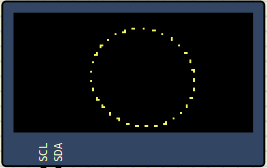
\includegraphics[width=\linewidth]{Exp-3/signal_gen/1_1.png}
\\
\small (a) 1:1
\end{minipage}
\hfill
\begin{minipage}{0.23\textwidth}
\centering
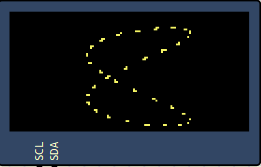
\includegraphics[width=\linewidth]{Exp-3/signal_gen/1_2.png}
\\
\small (b) 1:2
\end{minipage}
\hfill
\begin{minipage}{0.23\textwidth}
\centering
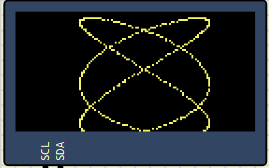
\includegraphics[width=\linewidth]{Exp-3/signal_gen/2_3.png}
\\
\small (c) 2:3
\end{minipage}
\hfill
\begin{minipage}{0.23\textwidth}
\centering
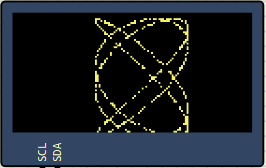
\includegraphics[width=\linewidth]{Exp-3/signal_gen/3_4.png}
\\
\small (d) 3:4
\end{minipage}

\caption{Different Lissajous Patterns Generated Using Various Frequency Ratios}
\label{fig:lissajous_output}

\end{figure}

%%%%%%%%%%%%%%%%%%%%%%%%%%%%%%%%%%%%%%%%%%%%%%%%%%%%%%%%%%%%%%%%%%%%%%%

\subsection{Conclusion}

The Arduino UNO Based Lissajous Pattern Generator was successfully implemented using dual sinusoidal inputs and an SSD1306 OLED display.

The system continuously sampled two analog signals, mapped them to X-Y coordinates, and generated various Lissajous figures in real time. The experiment provided a practical understanding of frequency ratio, phase difference, analog signal sampling, graphical visualization, and embedded graphics programming.

During this experiment, the following concepts were learned:

\begin{itemize}

\item Analog-to-Digital Conversion (ADC)

\item Signal sampling techniques

\item Coordinate mapping

\item Lissajous pattern generation

\item OLED graphics programming

\item Real-time signal visualization

\end{itemize}

%%%%%%%%%%%%%%%%%%%%%%%%%%%%%%%%%%%%%%%%%%%%%%%%%%%%%%%%%%%%%%%%%%%%%%%

\subsection{References}

\begin{enumerate}

\item Arduino Official Website

\url{https://www.arduino.cc/}

\item SSD1306 OLED Documentation

\url{https://github.com/adafruit/Adafruit_SSD1306}

\item Adafruit GFX Library

\url{https://github.com/adafruit/Adafruit-GFX-Library}

\item SimulIDE Official Website

\url{https://simulide.com/}

\item Lissajous Curves

\url{https://en.wikipedia.org/wiki/Lissajous_curve}

\end{enumerate}

%%%%%%%%%%%%%%%%%%%%%%%%%%%%%%%%%%%%%%%%%%%%%%%%%%%%%%%%%%%%%%%%%%%%%%%

\clearpage